\documentclass[tikz,border=5pt]{standalone}
\usepackage{amsmath}
\usepackage{pgfplots}
\pgfplotsset{compat=1.18}

\definecolor{corba}{HTML}{365FB3}
\definecolor{punt}{HTML}{B91C1C}
\definecolor{assimptota}{HTML}{6B7280}

\begin{document}
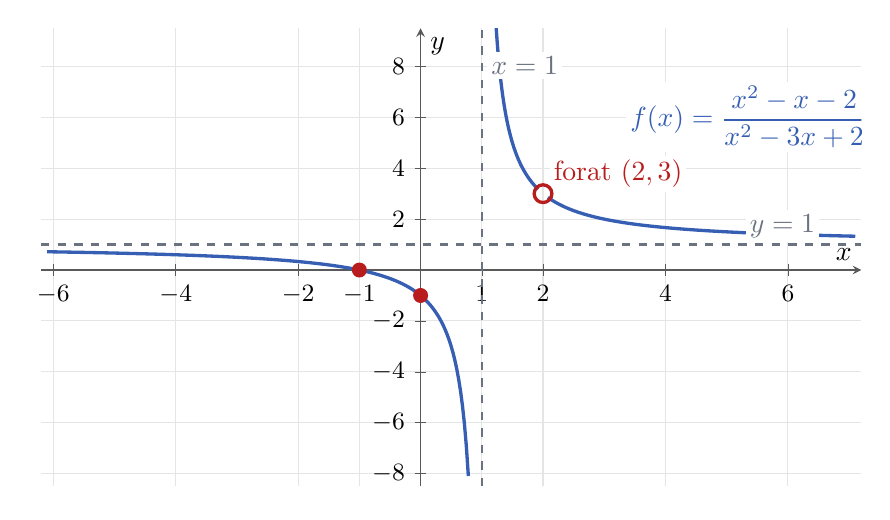
\begin{tikzpicture}
  \begin{axis}[
    width=12cm,
    height=7.4cm,
    axis lines=middle,
    xmin=-6.2,
    xmax=7.2,
    ymin=-8.5,
    ymax=9.5,
    xlabel={$x$},
    ylabel={$y$},
    xtick={-6,-4,-2,-1,0,1,2,4,6},
    ytick={-8,-6,-4,-2,0,2,4,6,8},
    grid=major,
    grid style={black!10},
    axis line style={black!65},
    tick style={black!65},
    tick label style={font=\small},
    clip=true,
  ]
    \addplot[assimptota, dashed, thick, domain=-6.2:7.2, samples=2] {1};
    \addplot[assimptota, dashed, thick] coordinates {(1,-8.5) (1,9.5)};

    \addplot[corba, very thick, domain=-6.1:0.78, samples=220]
      {(x+1)/(x-1)};
    \addplot[corba, very thick, domain=1.22:1.92, samples=100]
      {(x+1)/(x-1)};
    \addplot[corba, very thick, domain=2.08:7.1, samples=180]
      {(x+1)/(x-1)};

    \addplot[only marks, mark=*, mark size=2.5pt, punt]
      coordinates {(-1,0) (0,-1)};
    \addplot[
      only marks,
      mark=o,
      mark size=3.2pt,
      mark options={draw=punt, fill=white, line width=1.2pt}
    ] coordinates {(2,3)};

    \node[anchor=south west, text=assimptota, fill=white, inner sep=1.5pt]
      at (axis cs:5.3,1.08) {$y=1$};
    \node[anchor=south west, text=assimptota, fill=white, inner sep=1.5pt]
      at (axis cs:1.08,7.5) {$x=1$};
    \node[anchor=south west, text=punt, fill=white, inner sep=1.5pt]
      at (axis cs:2.1,3.05) {forat $(2,3)$};
    \node[anchor=south west, text=corba, fill=white, inner sep=1.5pt]
      at (axis cs:3.35,4.6) {$f(x)=\dfrac{x^2-x-2}{x^2-3x+2}$};
  \end{axis}
\end{tikzpicture}
\end{document}
